\documentclass[a4paper,11pt]{article}
\usepackage{amsmath,amsthm,amsfonts,amssymb,amscd,amstext,vmargin,graphics,graphicx,tabularx,multicol} 
\usepackage[francais]{babel}
\usepackage[utf8]{inputenc}  
\usepackage[T1]{fontenc} 
\usepackage{pstricks-add,tikz,tkz-tab,variations}
\usepackage[autolanguage,np]{numprint} 

\setmarginsrb{1.5cm}{0.5cm}{1cm}{0.5cm}{0cm}{0cm}{0cm}{0cm} %Gauche, haut, droite, haut
\newcounter{numexo}
\newcommand{\exo}[1]{\stepcounter{numexo}\noindent{\bf Exercice~\thenumexo} : \marginpar{\hfill /#1}}
\reversemarginpar


\newcounter{enumtabi}
\newcounter{enumtaba}
\newcommand{\q}{\stepcounter{enumtabi} \theenumtabi.  }
\newcommand{\qa}{\stepcounter{enumtaba} (\alph{enumtaba}) }
\newcommand{\initq}{\setcounter{enumtabi}{0}}
\newcommand{\initqa}{\setcounter{enumtaba}{0}}

\newcommand{\be}{\begin{enumerate}}
\newcommand{\ee}{\end{enumerate}}
\newcommand{\bi}{\begin{itemize}}
\newcommand{\ei}{\end{itemize}}
\newcommand{\bp}{\begin{pspicture*}}
\newcommand{\ep}{\end{pspicture*}}
\newcommand{\bt}{\begin{tabular}}
\newcommand{\et}{\end{tabular}}
\renewcommand{\tabularxcolumn}[1]{>{\centering}m{#1}} %(colonne m{} centrée, au lieu de p par défault) 
\newcommand{\tnl}{\tabularnewline}

\newcommand{\trait}{\noindent \rule{\linewidth}{0.2mm}}
\newcommand{\hs}[1]{\hspace{#1}}
\newcommand{\vs}[1]{\vspace{#1}}

\newcommand{\N}{\mathbb{N}}
\newcommand{\Z}{\mathbb{Z}}
\newcommand{\R}{\mathbb{R}}
\newcommand{\C}{\mathbb{C}}
\newcommand{\Dcal}{\mathcal{D}}
\newcommand{\Ccal}{\mathcal{C}}
\newcommand{\mc}{\mathcal}

\newcommand{\vect}[1]{\overrightarrow{#1}}
\newcommand{\ds}{\displaystyle}
\newcommand{\eq}{\quad \Leftrightarrow \quad}
\newcommand{\vecti}{\vec{\imath}}
\newcommand{\vectj}{\vec{\jmath}}
\newcommand{\Oij}{(O;\vec{\imath}, \vec{\jmath})}
\newcommand{\OIJ}{(O;I,J)}


\newcommand{\bmul}[1]{\begin{multicols}{#1}}
\newcommand{\emul}{\end{multicols}}

\newcommand{\reponse}[1][1]{%
\multido{}{#1}{\makebox[\linewidth]{\rule[0pt]{0pt}{20pt}\dotfill}
}}

\newcommand{\titre}[5] 
% #1: titre #2: haut gauche #3: bas gauche #4: haut droite #5: bas droite
{
\noindent #2 \hfill #4 \\
#3 \hfill #5

\vspace{-1.6cm}

\begin{center}\rule{6cm}{0.5mm}\end{center}
\vspace{0.2cm}
\begin{center}{\large{\textbf{#1}}}\end{center}
\begin{center}\rule{6cm}{0.5mm}\end{center}
}



\begin{document}
\pagestyle{empty}
\titre{Contrôle 1}{Nom :}{Prénom :}{Classe}{Date}



\exo{5}  Nombres relatifs\\

\begin{tabular}{|c|c|c|c|c|c|c|c|c|c|c|}
\hline 
Réponses & \hspace*{1cm} & \hspace*{1cm} & \hspace*{1cm} & \hspace*{1cm} & \hspace*{1cm} &\hspace*{1cm}  & \hspace*{1cm} & \hspace*{1cm} & \hspace*{1cm} & \hspace*{1cm} \\ 
\hline 
\end{tabular} \\



\exo{3} Cours \\

\noindent 
\q Énoncer clairement le théorème de Pythagore\\
\q Énoncer clairement la réciproque du théorème de Pythagore\\
\q Écrire l'égalité donnée par le théorème de Pythagore dans le cas suivant : soit TRS un triangle rectangle en R. \\




\exo{3}

\bmul{2}

\initq 
\q Donner la valeur arrondi au millimètre près de la longueur de AC : (Justifier votre réponse)\\

\includegraphics[scale=1]{pythago.eps} 

\columnbreak

\q Le triangle ABC est-il rectangle ? (Justifier votre réponse)

\includegraphics[scale=1]{pythagore.eps} 

\emul

\exo{4} En utilisant les informations sur les figures, calculer la longueur AC. (Justifier votre réponse)\\

\includegraphics[scale=1]{pyth1.eps} 


\exo{2}\\

\bmul{2}

Cet arbuste, qui vient d'être planté sur un terrain supposé horizontal a été haubané par un câble long de 2,50 m fixé sur le tronc à 1,40 m du sol et au sol à 2 m du pied de l'arbuste. Cet arbuste est-il bien vertical ?

\columnbreak


\begin{center}

\includegraphics[scale=1]{arbre.eps} 
\end{center}
\emul

\exo{3}\\
\bmul{2}
A partir des information potées sur le dessin suivant, démontrer que les droites (EF) et (FG) sont perpendiculaires.

\columnbreak

\includegraphics[scale=1]{difficicel.eps} 
\emul



\exo{} Bonus\\

Est-il possible de poster cette lettre rectangulaire sans la plier ?\\

\begin{center}

\includegraphics[scale=1]{timbre.eps} 
\end{center}

\end{document}
